\documentclass{beamer}
\usepackage{amsmath,amssymb,amsthm,array}
\usepackage{bm}
\usepackage{multirow}
\usepackage{multicol}
\usepackage{algorithm}
\usepackage{hyperref}
\usepackage{algorithmic}
\usepackage[normalem]{ulem}
\usepackage{fontspec}
\usepackage{numprint}

\setmainfont{CMU Serif}
\setsansfont{CMU Sans Serif}
\newfontfamily{\greekfont}{CMU Serif}
\newfontfamily{\greekfontsf}{CMU Sans Serif}

\usetheme{metropolis}
 
\setbeamertemplate{navigation symbols}{}
\title{Ψηφιακές Υπογραφές}
\author{Παναγιώτης Γροντάς - Άρης Παγουρτζής}
\date{27/11/2018}
\defbeamertemplate*{footline}{shadow theme}
{%
  \leavevmode%
  \hbox{
		\begin{beamercolorbox}[wd=.4\paperwidth,ht=2.5ex,dp=1.125ex,leftskip=.3cm,rightskip=.3cm plus1fil]{title in head/foot}%
			\usebeamerfont{title in head/foot} Digital Signatures  %
		\end{beamercolorbox}
		\begin{beamercolorbox}[wd=.5\paperwidth,ht=2.5ex,dp=1.125ex,leftskip=.3cm,rightskip=.3cm plus1fil]{title in head/foot}%
			\usebeamerfont{title in head/foot} \hfill \insertsection  %
		\end{beamercolorbox}
		\begin{beamercolorbox}[wd=.1\paperwidth,ht=2.5ex,dp=1.125ex,leftskip=.3cm plus1fil,rightskip=.3cm]{author in head/foot}%
			\usebeamerfont{author in head/foot}\insertframenumber\,/\,\inserttotalframenumber
		\end{beamercolorbox}%
  }%
  \vskip0pt%
}
\institute{ΕΜΠ - Κρυπτογραφία (2018-2019)}

 \hypersetup{
  pdfauthor={Panagiotis Grontas},
  pdftitle={DS},
  colorlinks=true,
  urlcolor=blue,
  pdfborderstyle={/S/U/W 1}	% border style will be underline of width 1pt
}

\setlength{\columnseprule}{0.4pt}
\begin{document}
\newcommand{\xor}{ \oplus }
\newcommand{\msg}{ \mathtt{M} }
\newcommand{\KEY}{ \mathtt{K} }
\newcommand{\CPH}{ \mathtt{C} }
\newcommand{\keygen}{\mathtt{KeyGen}}
\newcommand{\enc}{\mathtt{Encrypt}}
\newcommand{\dec}{\mathtt{Decrypt}}
\newcommand{\sign}{\mathtt{Sign}}
\newcommand{\verify}{\mathtt{Verify}}
\newcommand{\adv}{$\mathcal{A}$ }
\newcommand{\Hash}{\mathcal{H} }
\newcommand{\advb}{$\mathcal{B}$ }
\newcommand{\chal}{$\mathcal{C}$ }
\newcommand{\cs}{$\mathcal{CS}$}
\newcommand{\Zed}{\mathbb{Z}} 
\newcommand{\zns}{\mathbb{Z}^*_n}
\newcommand{\zs}[1]{\mathbb{Z}^*_{#1}}

\newcommand{\green}[1]{\textcolor{teal}{#1}}
\newcommand{\Green}[1]{\textcolor{Teal}{#1}}
\newcommand{\ForestGreen}[1]{\textcolor{ForestGreen}{#1}}
\newcommand{\blue}[1]{\textcolor{blue}{#1}}
\newcommand{\magenta}[1]{\textcolor{magenta}{#1}}
\newcommand{\cyan}[1]{\textcolor{cyan}{#1}}

\newcommand{\twopartdef}[4]
{ 
		\begin{cases}
			#1 , #2 \\
			#3 , #4
		\end{cases} 
}
\begin{frame}
\titlepage
\end{frame}

\begin{frame}{Περιεχόμενα}
\begin{itemize}
\item Ορισμός - Μοντελοποίηση Ασφάλειας
\item Ψηφιακές Υπογραφές RSA
\item Επιθέσεις - Παραλλαγές
\item Το μοντέλο του τυχαίου μαντείου
\item Ψηφιακές Υπογραφές ElGamal-DSA
\item Υποδομή Δημοσίου Κλειδιού
\end{itemize}
\end{frame}

\section{Εισαγωγή}
\begin{frame}{Εισαγωγή - Το πρόβλημα}
\begin{center}
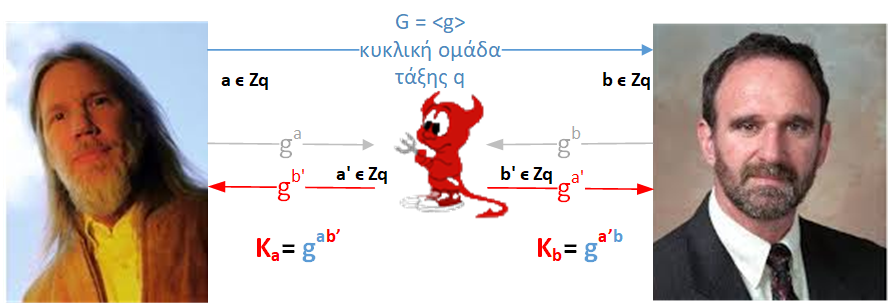
\includegraphics[scale=0.5]{dh-mitm.png}
\end{center}
\pause
Αποφυγή MITM attacks σε DHKE
\begin{itemize}
\item \textbf{Ακεραιότητα}: Το μήνυμα είναι \emph{αυτό} που έστειλε ο αποστολέας
\item \textbf{Αυθεντικοποίηση}: Το μήνυμα το έστειλε \emph{αυτός} που φαίνεται ως αποστολέας
\end{itemize}
\pause
Μία λύση: MACs
\alert{Μειονεκτήματα συμμετρικής κρυπτογραφίας}
\end{frame}

\begin{frame}{Ψηφιακές υπογραφές-Ασύμμετρα MACs}
\begin{itemize}
\item Ο αποστολέας (υπογράφων $S$) εκτελεί αλγόριθμο $\keygen$ και παράγει τα $(key_{sign},key_{ver})$
\begin{itemize}
\item Το κλειδί επαλήθευσης πρέπει να είναι δημόσιο\\
\item Το κλειδί υπογραφής πρέπει να διατηρείται μυστικό\\
\end{itemize}
\item Δημοσιοποιεί το κλειδί επαλήθευσης (web site, κατάλογο)
\pause
\item Πριν την αποστολή `υπογράφει το μήνυμα' (με το $key_{sign}$) παράγοντας την υπογραφή $\sigma$
\pause
\item Αποστέλλει το ζεύγος $(m,\sigma)$
\begin{itemize}
\item Η υπογραφή \emph{εξαρτάται} από το μήνυμα
\item Η υπογραφή είναι άχρηστη χωρίς το μήνυμα
\end{itemize}
\pause
\item Ο παραλήπτης (επαληθεύων $V$) ελέγχει αν η υπογραφή που έλαβε είναι έγκυρη (με το $key_{ver}$)
\end{itemize}
\end{frame}

\begin{frame}{Πλεονεκτήματα}
 
\begin{itemize}
\item Εύκολη διανομή κλειδιού
\pause
\item Δημόσια Επαληθευσιμότητα
\begin{itemize}
\item Δεν επαληθεύει μόνο ο παραλήπτης
\item Δημόσιο κλειδί: Μπορεί να επαληθεύσει οποιοσδήποτε
\end{itemize}
\pause
\item Μη αποκήρυξη (non repudiation)
\begin{itemize}
\item Αντιμετώπιση εσωτερικού αντίπαλου που προσπαθεί να αρνηθεί τις υπογραφές του
\item Μαθηματική σχέση κλειδιών υπογραφής - επαλήθευσης
\end{itemize}
\pause
\item Επιπλέον λειτουργίες
\begin{itemize}
    \item Αυθεντικοποίηση χρηστών (λόγω \emph{κατοχής} του ιδιωτικού κλειδού)
    \pause
    \item Ανωνυμία (τυφλές υπογραφές)
    \pause
    \item Αντιπροσωπεία από ομάδα (ομαδικές υπογραφές)
    \item ...
\end{itemize}
\end{itemize}
\end{frame}

\begin{frame}{Μειονεκτήματα}

Λύσαμε τα πρόβληματα \textbf{διανομής} κλειδιού, \textbf{αυθεντικότητας} και \textbf{ακεραιότητας} μηνύματος

Δημιουργήσαμε το πρόβλημα \textbf{αυθεντικότητας} κλειδιού

\begin{itemize}
\item \alert{Πώς είμαστε σίγουροι πως το ζεύγος κλειδιών αντιστοιχεί όντως στον $S$;}
\pause
\item \alert{Πώς είμαστε σίγουροι πώς το $key_{sign}$ ήταν στην κατοχή του $S$ κατά τη δημιουργία της υπογραφής;}
\end{itemize}
 
\pause Μαθηματικές και μη λύσεις
\end{frame}

\begin{frame}{Ορισμός}
\begin{block}{Σχήμα Υπογραφής}
Μια τριάδα από αλγόριθμους
\begin{itemize}
\item $\keygen(1^\lambda) = (key_{sign},key_{ver})$
\pause
\item $\sign(key_{sign}, m) = \sigma, \quad\quad m \in \{0,1\}^*$
\pause
\item $\verify(key_{ver}, m, \sigma) \in \{0,1\}$
\end{itemize}
\end{block}
\pause
\begin{block}{Ορθότητα}
$\verify(key_{ver}, m, \sign(key_{sign}, m))=1$
\end{block}
\pause
\green{Έγκυρες} υπογραφές: ικανοποιούν την απαίτηση της ορθότητας

\end{frame}

\begin{frame}{Επιθέσεις}
\begin{block}{Πλαστογραφία(Forgery)}
O \adv με δεδομένα το δημόσιο κλειδί επαλήθευσης και ένα μήνυμα παράγει μια έγκυρη υπογραφή χωρίς την συμμετοχή του $S$. 
\end{block}
\pause
\begin{block}{\alert{Είδη Επιθέσεων}}
\begin{itemize}
\item \alert{Καθολική πλαστογράφηση}: Ο \adv μπορεί να παράγει έγκυρες υπογραφές σε όποιο μήνυμα θέλει ($\Leftrightarrow$ κατοχή ιδιωτικού κλειδιού)
\pause
\item \alert{Επιλεκτική πλαστογράφηση}: Ο \adv μπορεί να παράγει 1 έγκυρη υπογραφή σε μήνυμα (με νόημα) της επιλογής του   
\pause
\item \alert{Υπαρξιακή πλαστογράφηση}: Ο \adv μπορεί να παράγει 1 έγκυρη υπογραφή (τυχαία bits) σε τυχαίο μήνυμα
\end{itemize}
\end{block}
\end{frame}

\begin{frame}[allowframebreaks]{Αντίπαλοι}
\begin{block}{Είδη Αντιπάλων}
\begin{itemize}
\item Παθητικός (passive): Απλά γνωρίζει το κλειδί επαλήθευσης και ζεύγη μηνυμάτων, έγκυρων υπογραφών
\item Ενεργός (active): Μπορεί να αποκτήσει έγκυρες υπογραφές σε μηνύματα της επιλογής του
\item Ενεργός με προσαρμοστικότητα (adaptive active): Μπορεί να αποκτήσει έγκυρες υπογραφές σε μηνύματα της επιλογής του που εξαρτώνται από προηγουμενες έγκυρες υπογραφές
\end{itemize}
\end{block}
\framebreak
Ασφάλεια ως προς τον δυνατότερο αντίπαλο - γενικότερη επίθεση

\begin{block}{Ασφάλεια}
Ένα σχήμα υπογραφής είναι ασφαλές αν δεν επιτρέπει σε έναν ενεργό αντίπαλο με προσαρμοστικότητα να επιτύχει υπαρξιακή πλαστογράφηση 
\end{block}
\end{frame}


\begin{frame}{Ορισμός Ασφάλειας}
\begin{block}{Το παιχνίδι πλαστογράφησης $Forge-Game$}
\begin{itemize}
\item Ο $S$ εκτελεί τον αλγόριθμο $\keygen(1^\lambda)$ και παράγει τα $(pk,sk)$
\pause
\item Ο \adv έχει πρόσβαση σε ένα μαντειο υπογραφών $\sign(sk,\cdot)$ με το οποίο αποκτά ένα σύνολο έγκυρων υπογραφών $Q = \{(m_i, \sigma_i)\}$ \\
\pause
\green{γιατί στην `πραγματική ζωή` μπορεί να χρησιμοποιήσει παλιότερες υπογραφές}
\pause
\item O \adv επιλέγει ένα μήνυμα $m$ και παράγει το ζεύγος $(m, \sigma)$ 
\pause
\item Νίκη \adv: $Forge-Game(\mathcal{A}) = 1 \Leftrightarrow \verify(key_{ver}, m, \sigma)=1 \wedge (m, \sigma) \not \in Q$
\end{itemize}
\end{block}
\pause
O \adv κερδίζει το παιχνίδι αν $Pr[Forge-Game(\mathcal{A})=1] = non-negl(\lambda)$
\end{frame}

\section{Ψηφιακές Υπογραφές RSA}
\begin{frame} {Ψηφιακές Υπογραφές RSA}
 
\textbf{Δημιουργία Κλειδιών:}
$KeyGen(1^{\lambda}) = (d,(e,n))$
\begin{itemize}
\item $n=p \cdot q$, $p,q$ πρώτοι αριθμοί $\frac{\lambda}{2}$ bits
\item Επιλογή $e$ ώστε $gcd(e,\phi(n))=1$
\item $d = e^{-1} \pmod{\phi(n)}$ με EGCD
\end{itemize}
\pause
\textbf{Υπογραφή} - Αποκρυπτογράφηση
\begin{itemize}
\item $\sign(d, m) = m^d \bmod n$
\end{itemize}
\pause
\textbf{Επαλήθευση} - Κρυπτογράφηση
\begin{itemize}
\item $\verify((e,n), m, \sigma) = \ \ \ \sigma^e =_? m \pmod{n}$
\end{itemize} 
\pause
\begin{block}{Ορθότητα}
$\verify((e,n), m, m^d \bmod{n})= \ \ \  {m^d}^e = m \pmod{n}$
\end{block}
\pause
\alert{...αλλά καθόλου ασφάλεια}
\end{frame}

\begin{frame}{Επίθεση Χωρίς Μήνυμα (No message attack)}
\begin{itemize}
\item O \adv έχει στη διάθεση του δημόσιο κλειδί $(e,n)$
\pause
\item $Q = \emptyset$ - δεν υποβάλλονται μηνύματα για υπογραφή
\pause
\item Επιλογή τυχαίου $\sigma \in \zns$
\pause
\item `Kρυπτογράφηση' $\sigma$: $\sigma^e \bmod n = m$
\pause
\item Το ζεύγος $(m,\sigma)$ είναι έγκυρο και $\not \in Q$
\pause
\item O \adv κερδίζει με πιθανότητα 1
\end{itemize}

\alert{Έχει νόημα;} - \green{Ναι}, με επαναλήψεις μπορούν να βρεθούν $m$ όπου κάποια bits μπορεί να είναι έγκυρα τμήματα μηνυμάτων
\end{frame}

\begin{frame}{Επίθεση Επιλεγμένων Μηνυμάτων (Chosen message attack)}
\begin{itemize}
\item O \adv έχει στη διάθεση του δημόσιο κλειδί $(e,n)$ και θέλει να πλαστογραφήσει υπογραφή για $m \in \zns$
\pause
\item O \adv χρησιμοποιώντας το μαντείο \textbf{αποκτά τις υπογραφές} 2 μηνυμάτων $Q = \{ (m_1, \sigma_1), (\frac{m}{m_1}, \sigma_2) \}$ με $m_1 \in_R \zns $
\pause
\item Υπολογισμός $\sigma = \sigma_1  \sigma_2 = m_1^d (\frac{m}{m_1})^d = m ^ d \bmod{n}$
\pause
\item H $\sigma$ είναι έγκυρη υπογραφή για το $m$ και $\not \in Q$
\end{itemize}
\end{frame}

\begin{frame}[allowframebreaks]{RSA - FDH (Full Domain Hash)}
 

\textbf{Δημιουργία Κλειδιών:}
$KeyGen(1^{\lambda}) = (d,(e,n))$
\begin{itemize}
\item $n=p \cdot q$, $p,q$ πρώτοι αριθμοί $\frac{\lambda}{2}$ bits
\item Επιλογή $e$ ώστε $gcd(e,\phi(n))=1$
\item $d = e^{-1} \pmod{\phi(n)}$ με EGCD
\item \green{Χρήση δημόσια διαθέσιμης τυχαίας συνάρτησης $ \Hash : \{ 0,1 \}^* \rightarrow \zns$}
\end{itemize}
  
\textbf{Υπογραφή} 
\begin{itemize}
\item \green{Υπολογισμός $\Hash(m)$}
\item $\sign(d, m) = \Hash(m)^d \bmod n$
\end{itemize}
\textbf{Επαλήθευση}
\begin{itemize}
\item \green{Υπολογισμός $\Hash(m)$}
\item $\verify((e,n), m, \sigma) = \ \ \ \sigma^e =_? \Hash(m) \pmod{n}$
\end{itemize} 

\begin{block}{Ορθότητα}
$\verify((e,n), m, \Hash(m)^d)= \ \ \  {\Hash(m)^d}^e = \Hash(m) \pmod{n}$
\end{block}
Υλοποίηση: συνάρτηση σύνοψης με δυσκολία εύρεσης συγκρούσεων
 
Πλεονέκτημα: Μπορεί να χρησιμοποιηθεί για υπογραφή τυχαίων συμβολοσειρών και όχι μόνο στοιχείων του $\zns$\

\framebreak

\begin{itemize}
\item Επίθεση χωρίς μήνυμα
\begin{itemize}
\item Επιλογή τυχαίου $\sigma \in \zns$
\item Η `κρυπτογράφηση` δίνει τη σύνοψη $h=\sigma^e \bmod{n}$ - όχι το μήνυμα
\item Για το μήνυμα πρέπει να βρεθεί $m: \Hash(m) = h$
\item Δυσκολία αντιστροφής
\end{itemize}
\framebreak

\item Επίθεση επιλεγμένων μηνυμάτων
\begin{itemize}
\item O \adv έχει στη διάθεση του δημόσιο κλειδί $(e,n)$ και θέλει να πλαστογραφήσει υπογραφή για $m \in \zns$
\item O \adv χρησιμοποιώντας το μαντείο αποκτά τις υπογραφές 2 μηνυμάτων $Q = \{ (m_1, \sigma_1), (\frac{m}{m_1}, \sigma_2) \}$ με $m_1 \in_R \zns $
\item Υπολογισμός $\sigma = \sigma_1  \sigma_2 = \Hash(m_1) \Hash(\frac{m}{m_1}) $
\item Δυσκολία αντιστροφής
\end{itemize}
\end{itemize} 


\begin{itemize}
\item Απόδειξη Ασφάλειας: Πρέπει η $\Hash$ να δίνει 'τυχαίες΄ τιμές
\item Αρκούν οι ιδιότητες τους (one-way-ness, collision resistance); 
\begin{itemize}
\item \alert{ΟΧΙ}
\end{itemize}
\item Το μοντέλο του τυχαίου μαντείου (M. Bellare, P. Rogaway, -1993)
\end{itemize}
\end{frame}

 
\section{Το μοντέλο του τυχαίου μαντείου}

\begin{frame}{Συναρτήσεις σύνοψης ως τυχαίες συναρτήσεις - informal}
\begin{itemize}
\item Θεωρητικά θα θέλαμε να συμπεριφέρονται ως τυχαίες συναρτήσεις
\pause
\item Πρακτικά όμως:\alert{αδύνατον να κατασκευαστούν}
\pause
\begin{itemize}
\item Συνάρτηση $\Hash: \{0,1\}^n \rightarrow \{ 0,1 \}^{l(n)}$
\pause
\item Κατασκευή ως πίνακας τιμών: Απαιτούνται $2^n$ γραμμές
\begin{tabular}{|c|c|}
Έισοδος & Έξοδος \\
$0\cdots00$ & $r_1$ \\
$0\cdots01$ & $r_2$\\
$\cdots$ & $\cdots$\\
$1\cdots11$ & $r_{l(n)}$\\
\end{tabular}
\pause
\item Συμπίεση: Μείωση τυχαιότητας
\end{itemize}
\end{itemize}
\pause
Ακόμα και να μπορούσαν να κατασκευαστούν \\
αδύνατη αποθήκευση\\
εκθετική αποτίμηση (μη αποδεκτή και για χρήστη και για αντίπαλο)
\end{frame}

\begin{frame}[allowframebreaks]{Συναρτήσεις σύνοψης και αποδείξεις ασφάλειας}

\begin{block}{Τυχαίο Μαντείο - Αφαιρετική αναπαράσταση συνάρτησης σύνοψης}
\begin{itemize}
\item Μαύρο κουτί - απαντάει σε ερωτήσεις
\item (Τέλεια) Ασφάλεια στο κανάλι επικοινωνίας (μοντελοποίηση τοπικής αποτίμησης)
\item Είναι συνάρτηση (ίδια είσοδος - ίδια έξοδος σε κάθε κλήση)
\item Είναι συνάρτηση σύνοψης (υπάρχουν συγκρούσεις - αλλά είναι δύσκολο να βρεθούν)
\end{itemize}
\end{block}

\framebreak

\begin{block}{Lazy Evaluation}
\begin{itemize}
\item Εσωτερικός πίνακας - αρχικά άδειος
\item Για κάθε ερώτηση: έλεγχος αν έχει ήδη απαντηθεί
\item Αν ναι, τότε ανάκτηση της απάντησης
\item Αν όχι, απάντηση με τυχαία τιμή και αποθήκευση για μελλοντική αναφορά
\end{itemize}
\end{block}
\framebreak

Αποδείξεις στο μοντέλο τυχαίου μαντείου (Bellare - Rogaway)
\begin{itemize}
\item Ο \adv \emph{νομίζει} ότι αλληλεπιδρά με το τυχαίο μαντείο
\item Στην πραγματικότητα το προσομοιώνει η αναγωγή (programmability)
\item Μπορούμε να μάθουμε τις ερωτήσεις του \adv
\item Στο πραγματικό πρωτόκολλο το τυχαίο μαντείο αντικαθίσταται από μία πραγματική συνάρτηση (πχ. SHA256)
\end{itemize}

\framebreak

\end{frame}

\begin{frame}{Απόδειξη Ασφάλειας Hashed RSA}
\begin{theorem}
Αν το πρόβλημα RSA είναι δύσκολο, τότε οι υπογραφές Hashed RSA παρέχουν ασφάλεια έναντι πλαστογράφησης στο μοντέλο του τυχαίου μαντείου.
\end{theorem}
\pause
Γενική κατασκευή:
\begin{itemize}
\item Ο \adv μπορεί να κατασκευάσει πλαστογράφηση υπογραφής
\pause
\item Κατασκευή \advb που με χρήση του \adv και ενός τυχαίου μαντείου μπορεί να αντιστρέψει το RSA
\pause
\item \green{Είσοδος \advb}
\begin{itemize}
\item Δημόσιο κλειδί $(e,N)$
\pause
\item Στοιχείο $y \in \zns$
\pause
\end{itemize}
\item \magenta{Έξοδος \advb}
\begin{itemize}
\item $x=y^\frac{1}{e}$
\end{itemize}
\end{itemize}
\end{frame}


\begin{frame}[allowframebreaks]{Απόδειξη Ασφάλειας Hashed RSA \\ Επίθεση χωρίς μήνυμα} 

\begin{block}{Υπόθεση}
Για την πλαστογράφηση $(m,\sigma)$ έχει προηγουμένως ερωτηθεί στο μαντείο το $\Hash(m)$
\end{block}

\begin{block}{Συνέπεια}
Εφόσον η πλαστογράφηση είναι έγκυρη υπογραφή πρέπει $\sigma^e = \Hash(m)$
Άρα $\sigma = \Hash(m)^{\frac{1}{e}}$
\end{block}

\framebreak

\begin{itemize}
\item Ο \advb προωθεί το $(e,N)$ στον \adv
\item O \adv κάνει $q=poly(\lambda)$ ερωτήσεις στο μαντείο για μηνύματα $\{m_i\}_{i=1}^q$ και λαμβάνει τις απαντήσεις $\{\Hash(m_i)\}_{i=1}^q \in_r \zns$
\item Ο \advb επιλέγει \emph{τυχαία} μία ερώτηση και αντικαθιστά την απάντηση $\Hash(m_i^*)$ με το $y$
\item Ο \advb \emph{ελπίζει} ότι στο $\Hash(m_i^*)$ θα γίνει η πλαστογράφηση
\item Αν έχει δίκιο, τότε ο \adv εξάγει την πλαστογραφία $(m,\sigma)$ με πιθανότητα $\mathtt{p}$
\item Δηλαδή: $\sigma^e = y \Rightarrow \sigma = y^\frac{1}{e}$
\item Ο \advb προωθεί το $\sigma$ στην έξοδο
\item Με πιθανότητα επιτυχίας $\frac{\mathtt{p}}{q}$ θα ισχύει $\sigma = y^\frac{1}{e}$
\end{itemize}

\begin{center}
Αν $\mathrm{\mathtt{p}}$ αμελητέο τότε $\frac{\mathtt{p}}{q}$ αμελητέο
\end{center}

\framebreak
\begin{center}
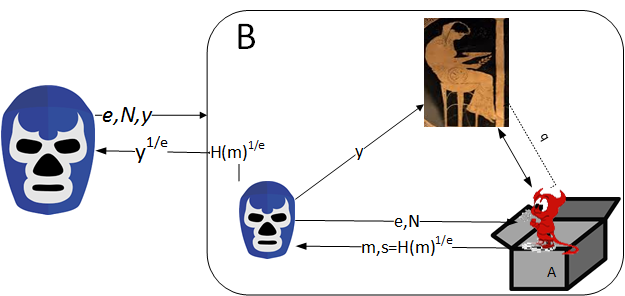
\includegraphics[scale=0.7]{ro-nom.png}
\end{center}
\end{frame}


\begin{frame}[allowframebreaks]{Απόδειξη Ασφάλειας Hashed RSA \\ Επίθεση επιλεγμένου μηνύματος} 

\begin{block}{Σενάριο}
\begin{itemize}
\item \adv πρέπει να υπολογίσει έγκυρες υπογραφές
\item Ζητάει συνόψεις και υπογραφές από τον \advb
\item Συνόψεις: το τυχαίο μαντείο
\item Υπογραφές: Πρέπει να τις απαντήσει ο \advb
\item ...χωρίς το ιδιωτικό κλειδί
\end{itemize}
\end{block}

\green{Λύση}

Αντικατάσταση $\Hash (m)$ με $\sigma^e$ για γνωστό $\sigma$

Τετριμμένη επαλήθευση $\sigma^e = \sigma^e (=\Hash(m))$



\framebreak
\begin{itemize}
\item Ο \advb προωθεί το $(e,N)$ στον \adv
\item O \adv κάνει $q$ ερωτήσεις στο μαντείο για μηνύματα $\{m_i\}_{i=1}^q$
\item Κάθε ερώτηση απαντάται από τον \advb ως εξής:
\begin{itemize}
\item Επιλέγει τυχαίο $\sigma_i \in \zns$
\item Υπολογίζει $y_i = \Hash(m_i) = \sigma_i^e \bmod N$
\item Επιστρέφει $y_i$
\item Aποθηκεύει τις  τριάδες $\mathcal{T} = (m_i, y_i, \sigma_i)$
\end{itemize}

\item O \adv ζητάει υπογραφές
\begin{itemize}
\item Για κάθε σύνοψη $y_i$ γίνεται αναζήτηση στον $\mathcal{T}$ για την τριάδα και επιστρέφεται το $\sigma_i$
\item Οι υπογραφές είναι έγκυρες αφού $\sigma_i^e = y_i$
\end{itemize}
\item Ο \advb μαντεύει ποιο ερώτημα στο RO θα οδηγήσει στην πλαστογράφηση.  Το απαντάει με $y$
\item Για το συγκεκριμένο δεν θα ζητηθεί υπογραφή, αλλά το $\sigma$ θα παραχθεί από τον \adv (πλαστογράφηση)
\item Για να είναι έγκυρη η πλαστογράφημενη υπογραφή πρέπει $\sigma^e = y$,δηλαδή $\sigma=y^\frac{1}{e}$
\item Πιθανότητα επιτυχίας \adv $p$ και πιθανότητα επιτυχίας \advb $\frac{p}{q}$
\end{itemize}

\begin{center}
Αν $\mathrm{\mathtt{p}}$ αμελητέο τότε $\frac{\mathtt{p}}{q}$ αμελητέο
\end{center}

\framebreak

\begin{center}
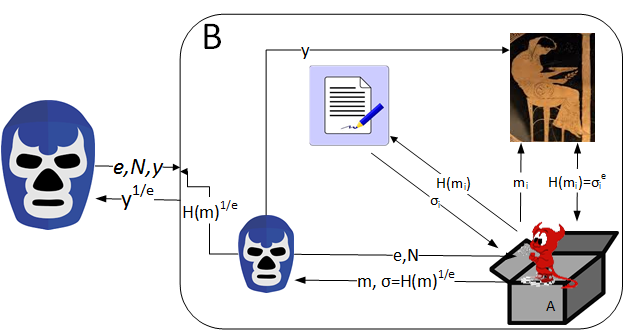
\includegraphics[scale=0.7]{ro-chosenm.png}
\end{center}

\end{frame}

\begin{frame}{Το μοντέλο του τυχαίου μαντείου - κριτική}
\begin{small}
\begin{block}{\alert{Μειονεκτήματα}}'Άχρηστη' απόδειξη - Καμία πραγματική συνάρτηση $\Hash$ δεν είναι random oracle \\
\pause
Εσωτερική χρήση - Δεν φαίνονται οι τιμές στις οποίες αποτιμάται \\
\pause
Programmability - Η περιγραφή της συνάρτησης είναι σταθερή στην πραγματικότητα \\
\pause
Ύπαρξη 'θεωρητικών' σχημάτων τα οποία αποδεικνύονται ασφαλή, αλλά οποιαδήποτε κατασκευή τους είναι μη ασφαλής \\
\end{block}
\pause
\begin{block}{\green{Πλεονεκτήματα}}
Απόδειξη με χρήση τυχαίου μαντείου είναι καλύτερη από απουσία απόδειξης \\
\pause
Η μόνη αδυναμία: η συνάρτηση σύνοψης \\
\pause
Δεν υπάρχουν πραγματικές επιθέσεις που να έχουν εκμεταλλευτεί την απόδειξη μέσω τυχαίου μαντείου
\end{block}
\end{small}
\end{frame}

\section{Ψηφιακές Υπογραφές ElGamal}

\begin{frame}[allowframebreaks]{Σχήμα Υπογραφής ElGamal}
 
\textbf{Δημιουργία Κλειδιών:}
\begin{itemize}  
\item Επιλογή πρώτου $p$. Δουλεύουμε στο $\zs{p}$ \alert{ΠΡΟΣΟΧΗ!}
\item Επιλογή γεννήτορα $g$
\item Επιλογή $x \in  \{2 \cdots p-2\}$ και υπολογισμός του $y = g^x \pmod{p}$
\item Δημόσιο κλειδί $(p,g,y)$, ιδιωτικό κλειδί $x$.
\end{itemize}
 
\textbf{Υπογραφή Μηνύματος $m$}
\begin{itemize}
\item Επιλογή τυχαίου $k \in \zs{p-1} \ δηλ. \ gcd(k,p-1)=1$
\item Υπολογισμός
\begin{align*}
r  =   g^k \bmod p \\
s  =   (m - x r) k^{-1} \bmod{(p-1)} 
\end{align*}

\item Υπογραφή είναι:$(r,s)$
\item Δύο ακέραιοι μεγέθους $O(|p|)$
\end{itemize}
\framebreak

\textbf{Επαλήθευση υπογραφής στο $m$}

$\verify(y,m,(r,s)) =\twopartdef{1}{\;\;\;\; y^r \cdot r^s \equiv g^m  \pmod{p}}{0}{\;\;\;\;  y^r \cdot r^s \neq g^m   \pmod{p}}$

\medskip

\begin{block}{Ορθότητα}
 
\begin{align*}
y^r r^s \equiv g^{xr} g^{ks} = g^{xr+ks} \equiv g^m\pmod{p}
\end{align*}

το οποίο ισχύει λόγω της κατασκευής του $s$
\end{block}

\end{frame}

\begin{frame}{Παρατηρήσεις}
\begin{itemize}
\item Πιθανοτικό σχήμα υπογραφής - πολλές έγκυρες υπογραφές για ένα μήνυμα $m$ (τυχαίο $k$)
\pause
\item Η συνάρτηση επαλήθευσης δέχεται οποιαδήποτε από αυτές ως έγκυρη
\pause
\item Χειρισμός Τυχαιότητας
\begin{itemize}
\item Το τυχαία επιλεγμένο $k$ πρέπει να κρατείται κρυφό
\item H επανάληψη της χρήσης του ίδιου $k$ καθιστά για τον \adv εφικτό τον υπολογισμό του  
\end{itemize}
\end{itemize}
\end{frame}

\begin{frame}{Επίθεση επανάληψης κλειδιού}
Χρήση ίδιου εφήμερου κλειδιού στην υπογραφή δύο μηνυμάτων $m_1,m_2$
\begin{itemize}
    \item $sign(x,m_1) = (r,s_1)$ με $s_1 = (m_1 - x r) k^{-1} $ \pause 
    \item $sign(x,m_2) = (r,s_2)$ με $s_2 = (m_2 - x r) k^{-1} $ \pause
    \item Υπολογισμός $s_1 - s_2 = (m_1 - m_2) k^{-1} \Rightarrow (s_1-s_2)k = (m_1-m_2)$ \pause 
    \item Δεν ισχύει γενικά $gcd(s_1 - s_2, p-1) = 1$ \pause
    \item Όμως υπάρχουν $gcd(s_1 - s_2,p-1)$ λύσεις για το $k$ (αν διαιρεί το $m_1 - m_2$)
    \item Δοκιμή όλων των πιθανών $g^k$ και σύγκριση με το γνωστό $r$ \pause
    \item Yπολογισμός ιδιωτικού κλειδιού από $rx = m_1 - ks_1$ \pause
    \item Δοκιμή όλων των $gcd(r,p-1)$ ως προς $y=g^x$ 
\end{itemize}
\end{frame}

\begin{frame}[allowframebreaks]{Ασφάλεια έναντι πλαστογράφησης}

\alert{Στόχος: $g^{xr} \cdot r^s \equiv g^{m} \pmod p$}

\begin{enumerate}
\item No message attack: Επιλέγω $r$ και $s$, ψάχνω $m$: Επίλυση DLP.

\item Chosen message attack: Επιλέγω $m$ και προσπαθώ να βρώ $r,s$ για έγκυρη υπογραφή
\begin{itemize}
\item Επιλέγω $r$, ψάχνω $s$. Πρέπει
$r^s \equiv g^{m} \cdot g^{-xr} \pmod p$ (επίλυση DLP).

\item Επιλέγω $s$, ψάχνω $r$. Πρέπει:
$g^{xr}  \equiv g^{m} \cdot r^{-s} \pmod p$

Ανοιχτό πρόβλημα - δε γνωρίζουμε σχέση με DLP 
\end{itemize}
 
 
\framebreak

\item Κατασκευή $r$, $s$, $m$ ταυτόχρονα.\\
Επιλέγω $i,j$
με $ \ \ 0\leq i,j \leq p-2, $\\
και $ \ \  \gcd(j,p-1)=1$  και θέτω: \\
\begin{align*}
 r=g^{i} \cdot (g^{x})^j \bmod p \\
 s = -r\cdot j^{-1} \bmod {p-1} \\
 m = -r\cdot i\cdot j^{-1} \bmod {p-1}
\end{align*}

\green {Τα (r,s) επαληθεύουν την υπογραφή}

\alert{Εφικτό σενάριο, δίνει υπογραφή για τυχαίο $m$}

\green{Aντιμετώπιση με redundancy function / hash function}

\end{enumerate}
 
\end{frame}

\begin{frame}
\frametitle{Πρότυπο Ψηφιακής Υπογραφής (Digital Signature Standard -- DSS)} 

\begin{block}{Βασικά Στοιχεία}
\begin{itemize}
\item NIST, 1991.
\pause
\item Παραλλαγή του ElGamal, μικρότερο μέγεθος υπογραφής.
\pause
\item Ιδέα: λειτουργία σε μια \magenta{υποομάδα της $\Zed_p^*$, τάξης $2^{160}$}.
\pause
\item Τα $r, s$ είναι εκθέτες δυνάμεων του γεννήτορα της υποομάδας.
\end{itemize}
\end{block}
\end{frame}


\begin{frame}
\frametitle{Παραγωγή κλειδιών DSS}

\begin{block}{}
\begin{enumerate}
\item Επιλογή πρώτων $q$ μεγέθους 160-bit και $p$ μεγέθους $n$-bit, $n=64{\lambda}$, $\lambda=8,9,10,\ldots,16$, με $q \mid (p-1)$.\pause
\item Εύρεση $g$ γεννήτορα της υποομάδας τάξης $q$ του $\mathbb{Z}_p^*$ \pause
\item Επιλογή ιδιωτικού κλειδιού $x \in \Zed_q$.\pause
\item Υπολογισμός $g^x \bmod{p}$. 
\end{enumerate}
\pause
\begin{flushleft}
Δημόσιο κλειδί: $(p,q,g,y), y = g^x \bmod p$.\\
Ιδιωτικό κλειδί: $x$.
\end{flushleft}
\end{block}

\end{frame}


\begin{frame} \frametitle{DSS:Δημιουργία υπογραφής}

\begin{block}{}
\begin{enumerate}
\item Ο υπογράφων επιλέγει έναν τυχαίο ακέραιο $k,\ 1 \leq k \leq (q-1)$.\pause
\item Υπολογίζει τα \pause
\begin{align*}
r  =   (g^k \bmod{p}) \bmod{q}  \\
s  =   (\Hash(m)+ x \cdot r)k^{-1}\bmod{q}
\end{align*} 
\item Αν συμβεί $r,s \equiv 0\pmod{q}$ η διαδικασία επαναλαμβάνεται \pause
\item Υπογραφή: $(r,s)$.
\end{enumerate}
\end{block}
\end{frame}


\begin{frame}\frametitle{DSS:Επαλήθευση υπογραφής DSA}
Ο $B$ υπολογίζει:

\begin{align*}
h=\Hash(m) \\
e_1  =   s^{-1} h \bmod{q} \\
e_2  =   rs^{-1}  \bmod{q} 
\end{align*}		 
\pause
\green{$\verify(y,m,(r,s)) = \mathsf{1} \Leftrightarrow (g^{e_1}(y)^{e_2} \bmod{p}) \bmod{q}=r$ }
\pause
\begin{block}{Ορθότητα}
\begin{align*}
g^{e_1}(y)^{e_2}  = 
g^{hs^{-1}} \cdot g^{xrs^{-1}}  \\
g^{hs^{-1}+xrs^{-1}}  = 
g^{(h+xr)s^{-1}} = \\
g^{kss^{-1}} = 
g^{k} (\bmod{p} \bmod{q})
\end{align*}
\end{block}
\pause
\alert{Υπογραφή γρηγορότερη από επαλήθευση}
\end{frame}

\section{Υποδομή Δημοσίου Κλειδιού}

\begin{frame}{Πρακτική χρήση ψηφιακών υπογραφών}
     \begin{itemize}
        \item Διαφορά Συμμετρικών - Ασύμμετρων Κρυπτοσυστημάτων
        \begin{itemize}
            \item Συμμετρικά: Δύσκολη διανομή, Εύκολη Αυθεντικότητα (λόγω φυσικών υποθέσεων)
            \item Ασύμμετρα: Εύκολη διανομή, Δύσκολη Αυθεντικότητα
        \end{itemize}
        \item Αντιστοιχία  (?) Ταυτότητας Χρήστη - Δημοσίου, Ιδιωτικού Κλειδιού (binding)
        \pause
        \item Ενεργός αντίπαλος - Πλαστοπροσωπία - αλλαγή κλειδιών
        \pause
        \item Απαραίτητη η διασφάλιση για χρήση σε ευρεία κλίμακα
        \pause
        \item \alert{Δεν υπάρχει λύση} που να δουλεύει θεωρητικά \textbf{και} πρακτικά
        \pause 
        \item Στην πράξη: μετάθεση του προβλήματος με μείωση της έκτασης (αρκεί 1 αυθεντικό κλειδί)
    \end{itemize}
\end{frame}

\begin{frame}{Αρχές Πιστοποίησης (Certification Authorities - CAs)}
    \begin{itemize}
    \item \emph{Έμπιστες} Τρίτες Οντότητες - (Πάροχοι Υπηρεσιών Πιστοποίησης)
    \pause
    \begin{itemize}
        \item Πιστοποίηση Αντιστοιχίας Ταυτότητας Κλειδιών
        \pause
        \item Εγγυάται ότι το δημόσιο κλειδί \emph{όντως} αντιστοιχεί στον χρήστη
        \pause
        \item Πώς;
        \pause 
        \item Υπογράφοντας `ψηφιακά` τo ζεύγος $(ID, PK_{ID})$        
    \end{itemize}
    \pause
    \item \green{Πλεονέκτημα}: Μείωση κλειδιών που πρέπει να αποκτήσουμε με έμπτιστο τρόπο
    \begin{itemize}
        \item Μόνο το κλειδί της CA
        \item Για τα υπόλοιπα `εγγύαται` το πιστοποιητικό
    \end{itemize}
    \item \alert{Μειονέκτημα} Ποιος εγγυάται την σχέση κλειδιών-ταυτότητας για την CA;
    \begin{itemize}
    \pause
    \item Η ίδια! (υπογράφει η ίδια μία δήλωση για τον εαυτό της)
    \pause
    \item ή μια άλλη \emph{ανώτερη} αρχή πιστοποίησης!
    \end{itemize}
    \end{itemize}
\end{frame}

\begin{frame}{Ιεραρχική Οργάνωση Αρχών Πιστοποίησης}
\begin{itemize} 
    \item Ενδιάμεσες Αρχές: Υπογραφή από ανώτερη αρχή 
    \item Ριζικές (Root) Αρχές: Υπογράφουν μόνες τους
    \item Συνήθως 3-4 επίπεδα
\end{itemize}
\begin{center}
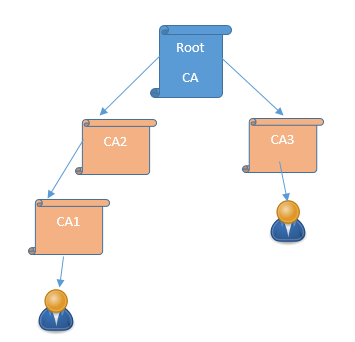
\includegraphics[scale=0.5]{pki.PNG}
\end{center}
\end{frame}

\begin{frame}{Υποδομή Δημοσίου Κλειδιού}
\begin{itemize}
    \item Οργάνωση των αρχών πιστοποίησης και των σχετικών υπηρεσιών \pause
    \item Loren Kohnfelder, MIT BSc thesis, 1978 \pause
    \item Ευρεία προτυποποίηση (ITU X.500, RFC 6818)
    \begin{itemize}
        \item Πρόσβαση σε υπηρεσίες καταλόγου
        \item X.509: Συσχέτιση οντότητας με δημόσιο κλειδί
        \item Ψηφιακό Πιστοποιητικό: 
        \begin{itemize}
            \item Δήλωση σχέσης κλειδιού - ονόματος
            \item Επιπλέον πληροφορίες για την επαλήθευση
        \end{itemize}
    \end{itemize}    
\end{itemize}
\end{frame}

\begin{frame}{Πιστοποιητικό X.509 - Δομή}
    \begin{center}
    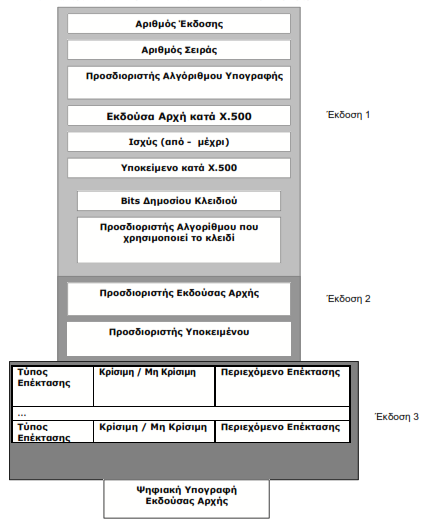
\includegraphics[scale=0.5]{x509.PNG}
    \end{center} 
\end{frame}

\begin{frame}{Πιστοποιητικό X.509 - Παράδειγμα} 
    \begin{tabular}{ c c }
    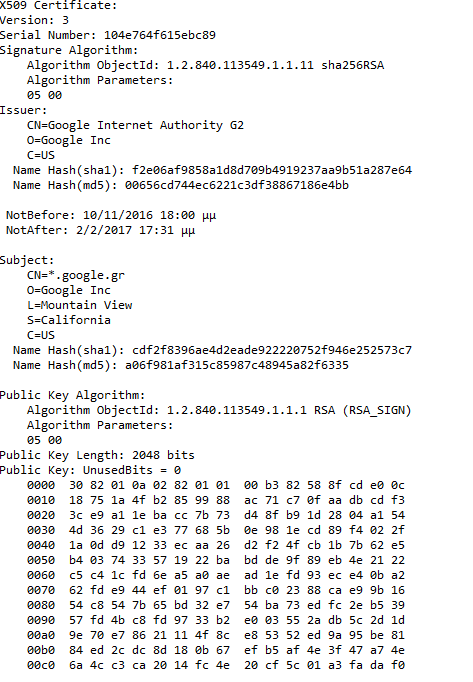
\includegraphics[scale=0.41]{cer1.PNG} & 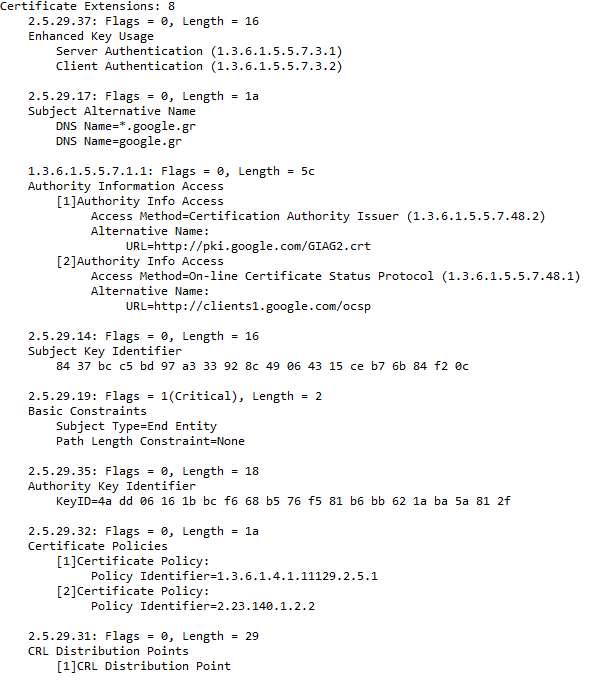
\includegraphics[scale=0.41]{cer2.PNG}
    \end{tabular}  
\end{frame}

\begin{frame}{Απόκτηση πιστοποιητικών}
\begin{itemize}
\item Προεγκατάσταση στο λειτουργικό σύστημα
\pause
\item Προεγκατάσταση στον περιηγητή
\pause
\item Απόκτηση από αρχείο/ιστοσελίδα
\pause
\item Απόκτηση από νομική οντότητα (εταιρεία, κράτος)
\pause
\end{itemize}
  \begin{center}
    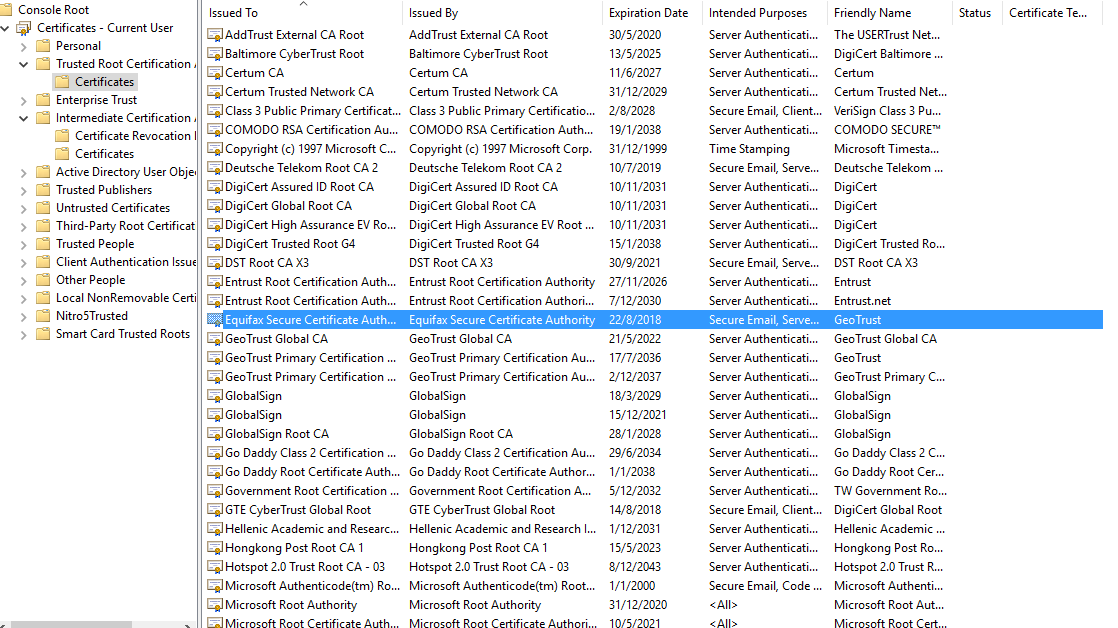
\includegraphics[scale=0.3]{certificates.PNG}
    \end{center} 
\end{frame}

\begin{frame}{Αρχές Πιστοποίησης - Άλλες υπηρεσίες}
    \begin{itemize}
        \item  Διάδοση Πιστοποιητικών σε αποθετήρια
        \pause
        \item  Εγγραφή-Επαλήθευση Ταυτότητας Χρηστών 
        \pause
        \item  Δημιουργία κρυπτογραφικών κλειδιών (αυστηρές προδιαγραφές ασφάλειας)
        \pause
        \item  Ανάκληση Πιστοποιητικών - Ενημέρωση
        \pause
        \item  Χρονοσήμανση - Αρχειοθέτηση
    \end{itemize}
\end{frame}

\begin{frame}{Ανάκληση Πιστοποιητικών}
Άκυρα πιστοποιητικά
\begin{itemize}
\item Απώλεια κλειδιού υπογραφής, Αλλαγή Στοιχείων Υποκειμένου, 
\pause
\item Ενημέρωση Χρηστών με 2 τρόπους
\pause
\item Certificate Revocation Lists (CRL): 
\begin{itemize}
    \item `Μαύρη` λίστα από SN για πιστοποιητικά που δεν ισχύουν
    \item Υπογεγραμμένη από την CA
    \item Ανάκτηση σε τακτά χρονικά διαστήματα
    \item Πεδίο CDP 
\end{itemize}
\pause
\item OCSP (Online Certificate Status Protocol)
\begin{itemize}
    \item Ερώτηση στην CA για ισχύ πιστοποιητικού
    \item H CA συμμετέχει σε κάθε συναλλαγή
\end{itemize}
\end{itemize}
\end{frame}

\begin{frame}{Εναλλακτικές Προσεγγίσεις: web of trust}
Ομότιμη έκδοση και επαλήθευση ταυτότητας (web of trust)
\begin{itemize}
    \item Κάθε χρήστης είναι CA \pause
    \item Υπογράφει αντιστοιχίες που γνωρίζει \pause
    \item Λήψη πιστοποιητικών μόνο από γνωστούς χρήστες \pause
    \item O κάθε χρήστης `εγγυάται` για τους γνωστούς του \pause
    \item PGP
\end{itemize}
\end{frame}

\begin{frame}{Identity based cryptography}
\begin{itemize}
    \item Signatures:Shamir 1984 \pause
    \item Encryption:Boneh-Franklin (2001) \pause
    \item Οποιοδήποτε όνομα κάποιου χρήστη πχ. email είναι η ταυτότητα \pause
    \item Δεν χρειάζεται διανομή κλειδιού \pause
    \item Χρειάζεται κεντρική TTP \pause
    \item Παράγει τα ιδιωτικά κλειδιά από την ταυτότητα \pause
\end{itemize}
\end{frame}

\begin{frame}{Identity based signatures}
\begin{itemize}
    \item TTP έχει κλειδί RSA $((e,n),d)$ \pause
    \pause
    \item Δημιουργία ιδιωτικού κλειδιού από ταυτότητα χρήστη $id$ \pause
    \pause
    \begin{itemize}
        \item Υπογραφή σύνοψης της ταυτότητας \pause
        \item $k = \mathcal{H}(id)^d \bmod{n}$ \pause
        \item Ασφαλής Διανομή στον κάτοχο \pause
    \end{itemize}
    \item Υπογραφή από χρήστη $id$ 
    \pause
    \begin{itemize}
        \item Επιλογή τυχαίου $r$ \pause
        \item $t =r^e \bmod{n}$  \pause
        \item $s =k \ r^{\mathcal{H}(m | t)} \bmod{n}$ \pause
        \item Η υπογραφή είναι $(t,s)$ 
    \end{itemize}
    \pause
    \item Επαλήθευση υπογραφής με την ταυτότητα:
    \pause
    \item Έλεγχος αν: $\mathcal{H}(id) t^{\mathcal{H}(m|t)} = s^e$ 
    \pause
    \item Ορθότητα: $\mathcal{H}(id) t^{\mathcal{H}(m|t)} = k^e r^{e\mathcal{H}(m|t)} = s^e$
\end{itemize}
\end{frame}


\begin{frame}[allowframebreaks]{Βιβλιογραφία}

\begin{tiny}
\begin{enumerate}
\item \href{http://hdl.handle.net/11419/5439}{Παγουρτζής, Α., Ζάχος, Ε., ΓΠ, 2015. Υπολογιστική κρυπτογραφία. [ηλεκτρ. βιβλ.] Αθήνα:Σύνδεσμος Ελληνικών Ακαδημαϊκών Βιβλιοθηκών}
\item Jonathan Katz and Yehuda Lindell. Introduction to Modern Cryptography (Chapman and Hall/Crc Cryptography and Network Security Series). Chapman
and Hall/CRC, 2007
\item Paar, Christof, and Jan Pelzl. Understanding cryptography: a textbook for students and practitioners. Springer Science-Business Media, 2009.
\item Kiayias, Aggelos  \href{http://crypto.di.uoa.gr/class/Kryptographia/Semeioseis_files/Cryptograph_Primitives_and_Protocols.pdf}{Cryptography primitives and protocols}, UoA, 2015
\item \href{http://goo.gl/b75I29}{Nigel Smart. Introduction to cryptography} 
\medskip
\item M. Green \href{http://blog.cryptographyengineering.com/2011/09/what-is-random-oracle-model-and-why.html}{What is the Random Oracle Model and why should you care?}
\item M. Bellare, P. Rogaway, (1993). "Random Oracles are Practical: A Paradigm for Designing Efficient Protocols". ACM Conference on Computer and Communications Security: 62–73.
\item R. Canetti, O. Goldreich, and S. Halevi.  The random oracle methodology, revisited. Journal of the ACM, 51(4):557–594, 2004.
\end{enumerate}
\end{tiny}
\end{frame}

\end{document}
